\documentclass[tikz]{standalone}

\usepackage{mathtools}

% Math operators definition
\let\Im\relax
\DeclareMathOperator{\Im}{Im}
\let\Re\relax
\DeclareMathOperator{\Re}{Re}

\usetikzlibrary{decorations.pathmorphing}

% Define ranges
\def\rerange{5}
\def\imrange{4}

\begin{document}
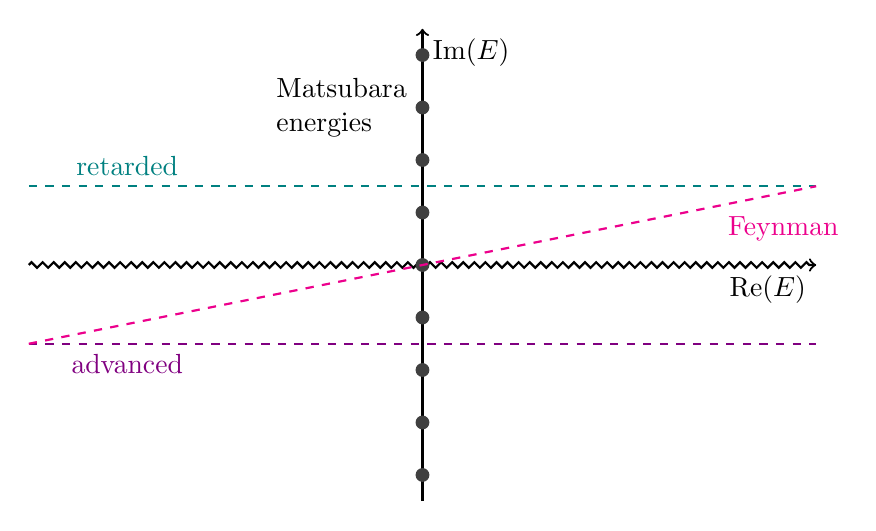
\begin{tikzpicture}[thick]

    % Axes (Modified: \omega -> E)
    \draw[->] [decorate, decoration={zigzag, segment length=4, amplitude=1, post=lineto, post length=2}] 
        (-\rerange, 0) -- (\rerange, 0) node[below left] {$\Re(E)$};
        
    \draw[->] (0, -\imrange+1) -- (0, \imrange-1) node[below right] {$\Im(E)$};

    % Matsubara Energies (Modified: fill color and label text)
    \foreach \n in {-\imrange, ..., \imrange}{%
        \node[circle, fill=darkgray, inner sep=0, minimum size=5] (energy\n) at (0, 2/3*\n) {};
    }
    \node[left=2, align=left] (mf) at (energy3) {Matsubara\\energies};

    % Propagators (Modified: colors)
    \draw[violet, dashed]  (-\rerange, -1) -- (\rerange, -1) node[below, very near start]       {advanced};
    \draw[teal, dashed]    (-\rerange, 1)  -- (\rerange, 1)  node[above, very near start]       {retarded};
    \draw[magenta, dashed] (-\rerange, -1) -- (\rerange, 1)  node[below right, very near end]   {Feynman};

\end{tikzpicture}
\end{document}